\begin{figure}
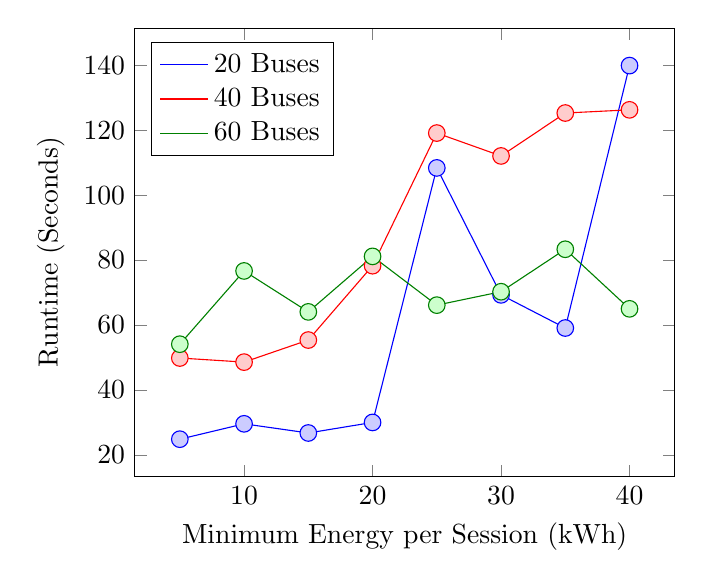
\begin{tikzpicture}
\begin{axis}[xlabel=Minimum Energy per Session (kWh), ylabel=Runtime (Seconds), legend pos=north west]
	\addplot[blue] coordinates {
		(5, 24.83)
	  (10,29.56)
		(15,26.74)
		(20,29.99)
		(25,108.38)
		(30,69.28)
		(35,59.07)
		(40,139.90)}; 
\addplot[red] coordinates {
		(5, 49.83)
	  (10,48.57)
		(15,55.37)
		(20,78.26)
		(25,119.12)
		(30,112.07)
		(35,125.29)
		(40,126.27)}; 
\addplot[green!50!black] coordinates {
		(5, 54.09)
	  (10,76.65)
		(15,64.04)
		(20,81.13)
		(25,66.12)
		(30,70.25)
		(35,83.33)
		(40,64.98)}; 
\addplot[blue!20, draw=blue, only marks, mark size=3pt] coordinates {
		(5, 24.83)
	  (10,29.56)
		(15,26.74)
		(20,29.99)
		(25,108.38)
		(30,69.28)
		(35,59.07)
		(40,139.90)}; 
\addplot[red!20, draw=red, only marks, mark size=3pt] coordinates {
		(5, 49.83)
	  (10,48.57)
		(15,55.37)
		(20,78.26)
		(25,119.12)
		(30,112.07)
		(35,125.29)
		(40,126.27)}; 
\addplot[green!20, draw=green!50!black, only marks, mark size=3pt] coordinates {
		(5, 54.09)
	  (10,76.65)
		(15,64.04)
		(20,81.13)
		(25,66.12)
		(30,70.25)
		(35,83.33)
		(40,64.98)}; 
\legend{20 Buses, 40 Buses, 60 Buses}		
\end{axis}
\end{tikzpicture}
\caption{Comparison of runtimes for various defragmentation scenarios in a pro-session environment}
\label{fig:results:defragmentationTimeProSchedule}
\end{figure}
